\documentclass[10pt,c,aspectratio=1610,handout]{beamer}
\usetheme[block=fill,numbering=fraction,progressbar=frametitle]{metropolis}
%\usecolortheme{beaver}
\usepackage{textpos}
\usepackage{amsmath}
\usepackage{amssymb}
\usepackage{appendixnumberbeamer}
\usepackage{caption}
\usepackage{subcaption}

\setbeamercovered{transparent}

\newcommand\blfootnote[1]{%
  \begingroup
  \renewcommand\thefootnote{}\footnote{#1}%
  \addtocounter{footnote}{-1}%
  \endgroup
}

\renewcommand{\baselinestretch}{1.25}
% Colour theme
\definecolor{QDMblue}{rgb}{0.00, 0.1882, 0.3608}
\definecolor{QDMgold}{rgb}{0.9098, 0.6510, 0.0000}
\definecolor{QDMgreen}{rgb}{0.3098, 0.5490, 0.0510}
\setbeamercolor{normal text}{ fg= QDMblue , bg= white }
\setbeamercolor{alerted text}{ fg= QDMgold }
\setbeamercolor{example text}{ fg= QDMgreen }

\begin{document}

% Personal Info
\title{Growth vs trend model handout}
\author[Konstantin Gantert]{\begin{large} Konstantin Gantert \end{large} \\ \textbf{Quantitative Dynamic Macroeconomics}}
\date{\textit{this version:} \today}

% Eliminates Navigation Bar on every Frame
\beamertemplatenavigationsymbolsempty

%-------------------------------------------------------------------------
% 0.1 Titlepage
%-------------------------------------------------------------------------
{\setbeamertemplate{footline}{} 
\frame{\titlepage}}
 \addtocounter{framenumber}{-1}
%-------------------------------------------------------------------------
% BLOCK: Growth vs. Trend Models
%-------------------------------------------------------------------------
\section{Growth vs. Trend Models}
%-------------------------------------------------------------------------
% The Growth Shock Model
\begin{frame}{The Growth Shock Model}%
  There are \textbf{two major stochastic models} of shocks that are used empirically.%
  \pause%
  \begin{itemize}%
    \item[$\blacktriangleright$] The first is the \textbf{growth shock model} in which%
    \begin{itemize}%
      \item[$\rightarrow$] Output follows $Y_t = (1+g_t)Y_{t-1}$  which means output in logs follows a random walk: \[ log(Y_t) = log(1+g_t) + log(Y_{t-1}) \approx y_t = g_t + y_{t-1} \]%
      \pause%
	    \item[$\rightarrow$] Hence over time the shocks build up linearly \[ y_t = \sum_{j=0}^{J-1} g_{t-j} + y_{t-J} \]%
	    \pause%
	    \item[$\rightarrow$] So the variance also grow linearly over time \[ var(y_t|y_{t-J}) = J \times \sigma^2 \]%
    \end{itemize}%
  \end{itemize}%
\end{frame}%
%-------------------------------------------------------------------------
% The Trend Stationary Model
\begin{frame}{The Trend Stationary Model}%
  \begin{itemize}%
    \item[$\blacktriangleright$] The second model is the \textbf{trend stationary model} in which changes have two parts:%
    \pause%
    \begin{itemize}%
      \item[$\rightarrow$] (i) a deterministic growth part $(1+g_t)$, and%
      \pause%
      \item[$\rightarrow$] (ii) a stationary stochastic part, typically an AR1 in logs, $X_t$.%
      \item[$\rightarrow$] Therefore, $Y_t = (1+g)^t \times X_t$ where \[ log(Y_t) = t \times g + log(X_t) \]%
      \item[$\rightarrow$] where \[ log(X_t) =x_t = \rho x_{t-1} + \sigma \epsilon_t \] where $\epsilon$ is a standard normal and $\rho \in [0,1)$.%
      \pause%
      \item[$\rightarrow$] This implies that \[ var(y_t) = var(x) = \sum_{j=0}^{\infty}\rho^{2j}  \sigma^2 = \frac{1}{1-\rho^2} \sigma^2 \]%
      \pause%
      \item[$\rightarrow$] And the conditional variance $J$ periods out is \[ var(x_t|x_{t-J}) = \sum_{j=0}^{J-1}\rho^{2j}  \sigma^2 = \frac{1-\rho^{2J}}{1-\rho^2} \sigma^2 \]%
    \end{itemize}%
  \end{itemize}%
\end{frame}%
%-------------------------------------------------------------------------
% What Happens to Growth Uncertainty?
\begin{frame}{What Happens to Growth Uncertainty?}%
  \begin{itemize}%
    \item[$\blacktriangleright$] \textbf{Stochastic growth model:} Uncertainty grows linearly with time.%
    \pause%
    \item[$\blacktriangleright$] \textbf{Trend stationary model:} Uncertainty shows a decreasing rate over time, largely dying out once we get enough away in time so that $\rho^J \approx 0$.%
    \pause%
    \item[$\blacktriangleright$] John Cochrane (JPE 1988) suggested we could use the behavior of the $k$th difference of log output to see how big the random walk component in output is:%
    \begin{itemize}%
      \item[$\rightarrow$] Assume that growth follows a combination of the two \[ Y_t = \sqrt{X_t Z_t} \] where $X_t$ is a stochastic trend term and $Z_t$ is stochastic growth component.%
      \item[$\rightarrow$] Taking logs gives us \[ y_t = (1/2) [ x_t + z_t ] \]%
    \end{itemize}%
  \end{itemize}%
\end{frame}%
%-------------------------------------------------------------------------
% Growth Shock vs. Trend Stationary
\begin{frame}{Growth Shock vs. Trend Stationary}%
  \begin{figure}[ht!]%
    \caption{Cochrane Measure of Unit Root vs. Simple Experiment}%
    \begin{center}%
    \subfloat[Data]{%
	    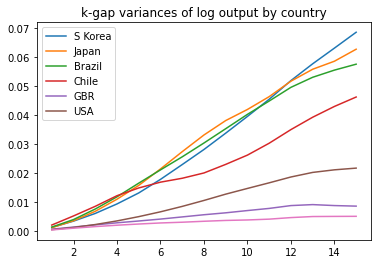
\includegraphics[scale=0.38]{figures/coch_fig1.png}}%
    \subfloat[Example]{%
	    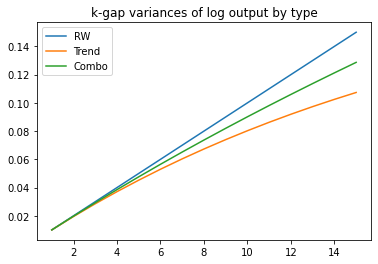
\includegraphics[scale=0.38]{figures/coch_fig2.png}}%
    \end{center}%
  \end{figure}%
  \begin{itemize}%
    \item[$\blacktriangleright$] Measure following Cochrane (1988); data: real GDP per capita, FRED; example: simulation.%
    \item[$\blacktriangleright$] Data for different countries suggests a large variation in the importance of a unit root.%
    \item[$\blacktriangleright$] However, the example figure suggests these differences are surprisingly subtle.%
  \end{itemize}%
\end{frame}%



%-------------------------------------------------------------------------
% References
\begin{frame}{References}%
  \begin{itemize}%
    \item[$\blacktriangleright$] Cochrane, John H. (1988). How big is the random walk in GNP?. Journal of political economy, 96(5), 893-920.%
    \item[$\blacktriangleright$] Cole, Harold L. (2020). Monetary and Fiscal Policy through a DSGE Lens. Oxford University Press.%
  \end{itemize}%
\end{frame}%
%-------------------------------------------------------------------------
\end{document}%